\section{实验分析}
\label{evaluation}

\subsection{实验设置}

在实验中我们采用了\emph{对照组},对照组作为比较的基准对象用最简易傻瓜的方式建模预测,具体地,$\hat y_{t+1} = y_t$,即用当天的实际头均采食量直接作为第二天的头均采食量预测值。
对照组的$\epsilon_{MAE}$(基准结果):1.1560。

我们采用交叉验证\footnote{具体地,$k$折交叉验证将所有数据样本随机平均分为$k$组,重复$k$次测试:每次测试用其中$k-1$组数据样本组合成训练集,训练构建得到模型(预测器),并将模型用于剩下的一组数据样本(作为测试集)进行预测,并在测试集上评估相关误差指标。}的方式评估模型的泛化能力,即对历史未见数据的预测能力。以下实验如不另加说明,均为8折交叉验证的结果。

在该节和附录中,我们用表格罗列出使用同种特征时,XGBoost模型选取各种不同参数(包括n\_enumerators和max\_depth)组合的结果。表格中的每一项a/b表示:在某种参数组合下,我们进行8折交叉验证的8次实验中,训练集上的$\epsilon_{MAE}$的平均值为a,测试集上的$\epsilon_{MAE}$的平均值为b。
我们用下划线突出标注每个表格中测试集上表现最优的结果。

%\begin{table}
%\caption{表格部分所用符号注解}
%\label{table_notation}
%\scriptsize
%\begin{center}
%\begin{tabular}{|c|p{5.6cm}|}
%\hline
%\textbf{符号} & \textbf{含义} \\
%\hline
%    THI & Thermal Humidity Index(温度湿度指数)。 \\
%    k & 回顾历史的天数。不加说明时,k=1。  \\
%    cA & 头均采食量时间序列做小波分解的1阶近似。 \\
%    cD & 头均采食量时间序列做小波分解的1阶细节。 \\
%    cA\_milk & 头均产奶量时间序列做小波分解的1阶近似。 \\
%    cD\_milk & 头均产奶量时间序列做小波分解的1阶细节。 \\
%    cA' & 头均采食量时间序列做小波分解的2阶近似。 \\
%    cD' & 头均采食量时间序列做小波分解的2阶细节。 \\
%\hline
%\end{tabular}
%\end{center}
%\end{table}%


\subsection{仅考虑单日数据}

表\ref{table_y_m}、\ref{table_y_m_thi}、\ref{table_y_m_thi_cald}、\ref{table_y_m_thi_cald_calp}是仅考虑当日数据,不考虑历史时序数据(w=1)的预测结果。
其中,表\ref{table_y_m}只考虑了头均采食量和头均产奶量两个特征,\ref{table_y_m_thi}、\ref{table_y_m_thi_cald}、\ref{table_y_m_thi_cald_calp}在该两个特征基础上,依次增加了温湿度指数(THI)、泌乳天数、泌乳期(胎次)特征。

观察表格可以发现:

(1) 就训练集而言,每组特征设置下,随着参数n\_enumerators和max\_depth的不断增大,训练集的误差不断减小。说明越复杂的模型可以越精确地刻划头均采食量的值。但是我们的目的是对未来的头均采食量做预测,我们需要关注模型的泛化性能,因而我们需要关注模型在测试集上的表现。

(2) 就测试集而言,每组特征设置下,在模型复杂度过低(参数n\_enumerators和max\_depth较小)或过高(参数n\_enumerators和max\_depth较大)时,测试集上的误差均相对较大,而在模型复杂度适中时,测试集上的误差相对较小。这说明过高的模型复杂度会导致过拟合现象,引起测试集上误差增大。我们可以通过比较测试集上的误差推断在某种特征设置下,什么是最合适的参数组合。

(3) 随着特征的不断丰富,测试集上的最小误差不断下降(由表\ref{table_y_m}中的1.168下降至\ref{table_y_m_thi_cald_calp}中的1.1014,说明增加的特征有助于模型更精准地刻划第二天的头均采食量。


\begin{table*}
\caption{头均采食量+头均产奶量}
\label{table_y_m}
\scriptsize
\begin{center}
	\begin{tabular}{|c|c|c|c|c|c|c|}
\hline
& \multicolumn{6}{|c|}{n\_enumerators} \\ \cline{2-7}
max\_depth & 75 & 100 & 150 & 200 & 250 & 300\\
\hline
1 & 1.1352/1.1788 & 1.1218/1.1722 & 1.1129/1.1691 & 1.1085/1.1686 & 1.1055/\wgs{1.168} & 1.1035/1.1681 \\
2 & 1.0972/1.1678 & 1.0863/1.1683 & 1.0692/1.1702 & 1.055/1.1718 & 1.0417/1.1749 & 1.0298/1.1776 \\
3 & 1.0627/1.1684 & 1.0451/1.1715 & 1.0161/1.1739 & 0.9879/1.18 & 0.9626/1.1864 & 0.9407/1.1947 \\
\hline
	\end{tabular}
\end{center}
\end{table*}%


\begin{table*}
\caption{头均采食量+头均产奶量+THI}
\label{table_y_m_thi}
\scriptsize
\begin{center}
	\begin{tabular}{|c|c|c|c|c|c|c|}
\hline
& \multicolumn{6}{|c|}{n\_enumerators} \\ \cline{2-7}
max\_depth & 75 & 100 & 150 & 200 & 250 & 300\\
\hline
1 & 1.1354/1.1794 & 1.1217/1.1716 & 1.1105/1.1684 & 1.1054/1.1678 & 1.1016/1.1671 & 1.0985/1.166 \\
2 & 1.0812/1.1526 & 1.0672/1.1498 & 1.0431/1.1452 & 1.0227/1.1426 & 1.0053/1.1397 & 0.9907/1.1388 \\
3 & 1.0284/1.1404 & 1.0019/1.1336 & 0.9587/1.1291 & 0.9239/\wgs{1.1277} & 0.894/1.1325 & 0.8668/1.1347 \\
4 & 0.9742/1.1415 & 0.9344/1.1329 & 0.8714/1.1288 & 0.8182/1.1311 & 0.7711/1.1366 & 0.7292/1.1423 \\
\hline
	\end{tabular}
\end{center}
\end{table*}%


\begin{table*}
\caption{头均采食量+头均产奶量+THI+泌乳天数}
\label{table_y_m_thi_cald}
\scriptsize
\begin{center}
	\begin{tabular}{|c|c|c|c|c|c|c|}
\hline
& \multicolumn{6}{|c|}{n\_enumerators} \\ \cline{2-7}
max\_depth & 75 & 100 & 150 & 200 & 250 & 300\\
\hline
1 & 1.1275/1.1739 & 1.1066/1.1591 & 1.0867/1.1474 & 1.0767/1.1431 & 1.0717/1.1419 & 1.0682/1.1416 \\
2 & 1.0512/1.1307 & 1.0335/1.1262 & 1.0078/1.124 & 0.9868/1.1187 & 0.9682/1.1187 & 0.9526/1.1195 \\
3 & 0.9884/1.1195 & 0.9595/1.1142 & 0.9116/1.1095 & 0.8733/1.1108 & 0.8391/1.1144 & 0.8088/1.1166 \\
4 & 0.9203/1.1086 & 0.8784/\wgs{1.1029} & 0.8068/1.1067 & 0.7481/1.1102 & 0.6973/1.1184 & 0.6521/1.1263 \\
5 & 0.8504/1.1032 & 0.79/1.1093 & 0.6967/1.12 & 0.6172/1.1312 & 0.5508/1.1443 & 0.4921/1.1507 \\
\hline
	\end{tabular}
\end{center}
\end{table*}%

\begin{table*}
\caption{头均采食量+头均产奶量+THI+泌乳天数+胎次}
\label{table_y_m_thi_cald_calp}
\scriptsize
\begin{center}
	\begin{tabular}{|c|c|c|c|c|c|c|}
\hline
& \multicolumn{6}{|c|}{n\_enumerators} \\ \cline{2-7}
max\_depth & 75 & 100 & 150 & 200 & 250 & 300\\
\hline
1 & 1.1266/1.1745 & 1.1066/1.1605 & 1.0873/1.1501 & 1.0775/1.1458 & 1.0724/1.1443 & 1.0686/1.1439 \\
2 & 1.0507/1.1341 & 1.0328/1.1273 & 1.0069/1.1233 & 0.9859/1.1207 & 0.9667/1.1167 & 0.9513/1.1158 \\
3 & 0.9867/1.1205 & 0.957/1.1134 & 0.9102/1.1103 & 0.8706/1.1094 & 0.8381/1.1092 & 0.8069/1.1126 \\
4 & 0.9192/1.106 & 0.875/\wgs{1.1014} & 0.8037/1.1029 & 0.7431/1.1052 & 0.6911/1.1108 & 0.6455/1.1137 \\
5 & 0.8435/1.1049 & 0.7807/1.1061 & 0.6858/1.1129 & 0.6047/1.1216 & 0.5376/1.1314 & 0.4801/1.141 \\
\hline
	\end{tabular}
\end{center}
\end{table*}%


\subsection{直接拼接多日时序数据}
\label{multiday_concat}

\begin{table}
\caption{直接拼接多日时序数据,测试集的$\epsilon_{MAE}$}
\label{table_total_concat}
\scriptsize
\begin{center}
	\begin{tabular}{|c|c|c|c|c|}
\hline
& \multicolumn{4}{|c|}{时间窗口大小 $w$} \\ \cline{2-5}
考虑时间序列的特征 & 2 & 3 & 4 & 5\\
\hline
头均采食量 & 1.1028 & 1.0993 & 1.091 & 1.0976 \\
头均产奶量 & 1.0979 & 1.0882 & \wgs{1.087} & 1.1007 \\
\hline
	\end{tabular}
\end{center}
\end{table}

本节和下一节我们考虑时间窗口大小w>1的情况,即我们在预测第二天的头均采食量时,除了考虑当天外,也考虑过去若干天的历史数据。在本节中,我们对多天历史数据采取直接拼接的处理方式。

表\ref{table_total_concat}概括列出了拼接不同时间序列时,测试集上的最优误差。具体实验结果请见附录第\ref{concat_exp_data}节中的表\ref{table_y2_m_thi_cald_calp}、\ref{table_y3_m_thi_cald_calp}、\ref{table_y4_m_thi_cald_calp}、\ref{table_y5_m_thi_cald_calp}和表\ref{table_y_m2_thi_cald_calp}、\ref{table_y_m3_thi_cald_calp}、\ref{table_y_m4_thi_cald_calp}、\ref{table_y_m5_thi_cald_calp}。


观察各表格可见考虑头均采食量和考虑头均产奶量历史数据得到的最优$\epsilon_{MAE}$比较接近(相差在均在0.012kg以内),在多个w取值(w=2,3,4)下,考虑头均产奶量历史数据实验得到的预测误差更小,且w取不同值时,测试集上最优的误差(1.087)在w=4,考虑头均产奶量历史数据时得到。




%
% Using wavelet decomposition
%
\subsection{小波分解考虑多日时序数据}
\label{multiday_dwt}

\begin{table}
\caption{一阶小波分解处理多日时序数据,测试集的$\epsilon_{MAE}$}
\label{table_total_dwt}
\scriptsize
\begin{center}
	\begin{tabular}{|c|c|c|c|c|}
\hline
& \multicolumn{4}{|c|}{时间窗口大小 $w$} \\ \cline{2-5}
考虑时间序列的特征 & 2 & 4 & 4(二阶) & 6\\
\hline
头均采食量 & 1.0851 & 1.0807 & 1.0858 & 1.0982 \\
头均产奶量 & 1.1016 & \wgs{1.0788} & 1.084 & 1.10939 \\
\hline
	\end{tabular}
\end{center}
\end{table}


本节我们同样考虑时间窗口大小w>1的情况。
本节中我们对多天头均采食量或头均产奶量历史数据的时间序列采取小波分解的方式提取特征。

表\ref{table_total_dwt}概括列出了对不同时间序列做不同处理时,测试集上的最优误差。具体实验结果请见附录第\ref{dwt_exp_data}节中的表\ref{table_wavelet_y2_m}、\ref{table_wavelet_y4_m}、\ref{table_wavelet_y4_2_m}、\ref{table_wavelet_y6_m}和表\ref{table_wavelet_y_m2}、\ref{table_wavelet_y_m4}、\ref{table_wavelet_y_m4_2}、\ref{table_wavelet_y_m6}。

观察各表格可见,与第\ref{multiday_concat}类似,考虑头均采食量和考虑头均产奶量历史数据得到的最优$\epsilon_{MAE}$比较接近(相差均在0.017kg以内),且在不同w取值下,两种考虑不同历史数据的方式的结果各有优劣,不存在绝对更优的一种历史数据处理方式。

测试集上最优的$\epsilon_{MAC}$(1.0788)在w=4,进行1层小波分解,考虑头均产奶量历史数据时得到。这也是\uline{所有实验中得到的最优结果}。和对照组的$\epsilon_{MAC}$(1.1560)相比,模型将预测头均采食量的平均绝对误差降低了$1.1560 - 1.0788=0.0772$。这意味着,XGBoost模型的预测和最简单的预测(用当天的头均采食量作为第二天头均采食量的预测值)相比,头均采食量的平均绝对误差下降了7.7\%千克。



\subsection{特征的重要程度}

图\ref{feature_importance}显示了最优结果($\epsilon_{MAE} = 1.0788$)对应的参数配置下(w=4,头均产奶量时间序列一层小波分解,max\_depth=4,n\_enumerator=100),一次交叉验证实验中,训练出的XGBoost模型调用函数plot\_importance\footnote{参见XGBoost的API文档:\url{http://xgboost.readthedocs.io/en/latest/python/python\_api.html\#module-xgboost.plotting}。}得到的各特征的权重。其中各编号对应的特征列举在表\ref{feature_desc}中。由于做8折交叉验证时训练出的8个模型得到的特征重要程度排序略有不同,我们综合考虑8次实验得到的8个特征排序,将特征按重要程度大致分为如下三组:076/214/538,其中权重最高的三个特征(076)为头均采食量、泌乳天数和THI,次高的三个特征(214)为:头均产奶量、小波分解的1阶近似和细节中各一个分量,最低的三个特征(538)为:小波分解的1阶近似和细节中各一个分量和胎次。

\begin{figure}
\begin{center}
	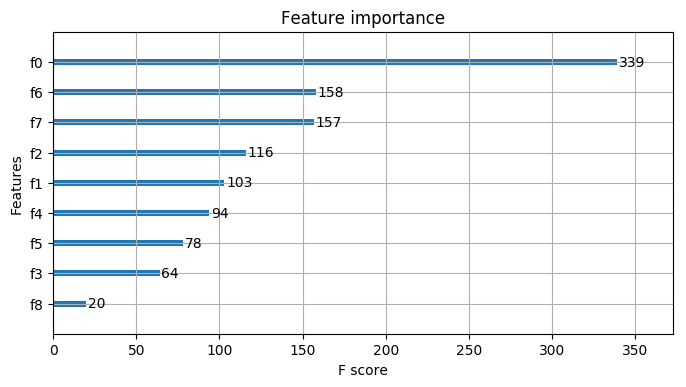
\includegraphics[width=0.95\linewidth]{feature_importance}
\caption{表\ref{table_total_concat}中最优结果对应的参数配置下,某次交叉验证中构建的回归树里各特征的权重。}
\label{feature_importance}
\end{center}
\end{figure}


\begin{table}
\caption{图\ref{feature_importance}中各编号对应的特征}
\label{feature_desc}
\footnotesize
\begin{center}
\begin{tabular}{|c|c|}
\hline
	特征编号	& 特征 \\
\hline
	f0 & $y_t$:头均采食量 \\
	f1 & $m_t$:头均产奶量\\
	f2, f3 & cA:小波分解1阶近似 \\
	f4, f5 & cD:小波分解1阶细节\\
	f6 & $T_{t+1}$:THI \\
	f7 & $cd_t$:泌乳天数 \\
	f8 & $cp_t$:胎次 \\
\hline
\end{tabular}
\end{center}
\end{table}%















